% !TEX root = ../main.tex
%

\part{正則化}\label{part:regularization}

\chapter{導入}

この章では,正則化のアルゴリズムをまとめる.

未知のパラメータ $\bm{x}$ に合わせて変動するデータ $\bm{y} = A \bm{x}$ をもとに
パラメータ $\bm{x}$ を推定する問題は一般に逆問題と呼ばれる.
ここで,$\bm{x}$, $\bm{y}$ はそれぞれ何らかのノルム空間 $X$, $Y$ に存在するベクトルで,
$A$ は何らかの作用素とする.
例えば,録音した音源をもとに音が鳴っている場所を調べたい場合,
音が鳴っている場所が $\bm{x}$ であり,
録音した音源は $\bm{y}$ になる.

逆問題を解く単純な手法として,
ノルム $\|A \bm{x} - \bm{y}\|$ の最小化(最小二乗法)が挙げられるが,
作用素 $A$ の性質によっては,
$\bm{y}$ が少し変動するだけで最小二乗法による解 $\bm{x}$ が大きく変動してしまう場合があったり,
解が複数存在してしまう場合があったりする(ill-posed problem と呼ばれる).
そのような場合に,追加の情報をもとに唯一の安定な解を求められるようにする手法を正則化と呼ぶ.
ここでは,特に次のような式を最小化する正則化手法における数値解法をまとめる.

\begin{equation}
    \|A \bm{x} - \bm{y}\|^2 + \lambda R(\bm{x})
    \label{eq:regularization_intro_general-regularization}
\end{equation}

ここで,$\lambda \in [0, \infty)$ は正則化パラメータと呼ばれるパラメータで,
$R$ は $R : X \to [0, \infty)$ のような関数である.
この式を最小化する解 $\bm{x}_{\lambda}$ は正則化パラメータ $\lambda$ により変化する.
$\lambda = 0$ では正則化の効果がなくなり,
$\lambda$ を大きくすると正則化の効果が強くなる.
$\lambda$ を大きくしすぎると残差 $\|A \bm{x} - \bm{y}\|^2$ が大きくなり,
データ $\bm{y}$ から離れていってしまうため,
正則化パラメータ $\lambda$ を適切に調整することが必要となる.

% !TEX root = ../main.tex
%

\chapter{Tikhonov 正則化}

ここでは基本的な Tikhonov 正則化についてまとめる.
Tikhonov 正則化では,評価関数
\begin{equation}
    E_{\lambda}(x) \equiv \|A \bm{x} - \bm{y}\|_2^2 + \lambda \|\bm{x}\|_2^2
    \label{eq:regularization_tikhonov_objective}
\end{equation}
を最小化する.
ここで,
$\bm{x} \in \setC^n$,
$\bm{y} \in \setC^m$,
$A \in \setC^{m \times n}$
である.

\begin{theorem}\label{theorem:regularization_tikhonov_solution}
    $\lambda > 0$ の場合,
    評価関数 \eqref{eq:regularization_tikhonov_objective} が最小となるのは,
    $\bm{x} = (A^* A + \lambda I)^{-1} A^* \bm{y}$ の場合である.
\end{theorem}
\begin{proof}
    この場合,ノルムを展開することで,次のようになる.
    \begin{align}
        E_{\lambda}(x)
         & = \|A \bm{x} - \bm{y}\|_2^2 + \lambda \|\bm{x}\|_2^2
        \notag                                                                                              \\
         & = (A \bm{x} - \bm{y})^* (A \bm{x} - \bm{y}) + \lambda \bm{x}^* \bm{x}
        \notag                                                                                              \\
         & = \bm{x}^* (A^* A + \lambda I) \bm{x} - \bm{x}^* A^* \bm{y} - \bm{y}^* A \bm{x} + \|\bm{y}\|_2^2
    \end{align}
    ここで,
    $\lambda > 0$ の場合は
    $\bm{x} \neq \bm{0}$ において
    $\bm{x}^* (A^* A + \lambda I) \bm{x} = \|A \bm{x}\|_2^2 + \lambda \|\bm{x}\|_2^2 > 0$
    となることから,
    エルミート行列 $(A^* A + \lambda I)$ は正定値であり,
    正則となる.
    このことを用いると,さらに次のように展開できる.
    \begin{align}
        E_{\lambda}(x)
         & = \bm{x}^* (A^* A + \lambda I) \bm{x} - \bm{x}^* A^* \bm{y} - \bm{y}^* A \bm{x} + \|\bm{y}\|_2^2
        \notag                                                                                              \\
         & = \bm{x}^* (A^* A + \lambda I) \bm{x} - \bm{x}^* A^* \bm{y} - \bm{y}^* A \bm{x}
        + \bm{y}^* A (A^* A + \lambda I)^{-1} A^* \bm{y}
        - \bm{y}^* A (A^* A + \lambda I)^{-1} A^* \bm{y}
        + \|\bm{y}\|_2^2
        \notag                                                                                              \\
         & = (\bm{x} - (A^* A + \lambda I)^{-1} A^* \bm{y})^*
        (A^* A + \lambda I)
        (\bm{x} - (A^* A + \lambda I)^{-1} A^* \bm{y})
        - \bm{y}^* A (A^* A + \lambda I)^{-1} A^* \bm{y}
        + \|\bm{y}\|_2^2
    \end{align}
    エルミート行列 $(A^* A + \lambda I)$ が正定値であることから,
    この式が最小となるのは
    $(\bm{x} - (A^* A + \lambda I)^{-1} A^* \bm{y})$
    が零ベクトルとなる場合,
    つまり,
    $\bm{x} = (A^* A + \lambda I)^{-1} A^* \bm{y}$
    の場合である.
\end{proof}

ここで,$\lambda = 0$ でも,行列 $A$ のランクが $n$ の場合は $A^*A$ が正定値になるため同様に解が求まる.

\section{特異値分解による解法}

行列 $A$ を次のように特異値分解する.

\begin{equation}
    A = U
    \begin{pmatrix}
        \Sigma & O \\
        O      & O
    \end{pmatrix}
    V^*
\end{equation}

ここで,$U \in \setC^{m \times m}$ と $V \in \setC^{n \times n}$ はユニタリ行列で,
$\Sigma \in \setR^{r \times r}$ は正の実数による対角行列である.
ただし,ランク $r$ は $m$ または $n$ に等しくても良い.

この分解を用いると,
定理 \ref{theorem:regularization_tikhonov_solution} の解は次のように変形できる.

\begin{align}
    x_{\lambda}
     & \equiv (A^* A + \lambda I)^{-1} A^* \bm{y}
    \notag                                        \\
     & = \left(V
    \begin{pmatrix}
        \Sigma & O \\
        O      & O
    \end{pmatrix}
    U^* U
    \begin{pmatrix}
        \Sigma & O \\
        O      & O
    \end{pmatrix}
    V^* + \lambda I \right)^{-1}
    V
    \begin{pmatrix}
        \Sigma & O \\
        O      & O
    \end{pmatrix}
    U^* \bm{y}
    \notag                                        \\
     & = \left(V
    \begin{pmatrix}
        \Sigma^2 & O \\
        O        & O
    \end{pmatrix}
    V^* + \lambda V V^* \right)^{-1}
    V
    \begin{pmatrix}
        \Sigma & O \\
        O      & O
    \end{pmatrix}
    U^* \bm{y}
    \notag                                        \\
     & = \left(V
    \begin{pmatrix}
        \Sigma^2 + \lambda I & O         \\
        O                    & \lambda I
    \end{pmatrix}
    V^* \right)^{-1}
    V
    \begin{pmatrix}
        \Sigma & O \\
        O      & O
    \end{pmatrix}
    U^* \bm{y}
    \notag                                        \\
     & = V
    \begin{pmatrix}
        (\Sigma^2 + \lambda I)^{-1} & O              \\
        O                           & \lambda^{-1} I
    \end{pmatrix}
    V^*
    V
    \begin{pmatrix}
        \Sigma & O \\
        O      & O
    \end{pmatrix}
    U^* \bm{y}
    \notag                                        \\
     & = V
    \begin{pmatrix}
        (\Sigma^2 + \lambda I)^{-1} \Sigma & O \\
        O                                  & O
    \end{pmatrix}
    U^* \bm{y}
\end{align}

さらに,
$U = (\bm{u}_1, \bm{u}_2, \ldots, \bm{u}_m)$,
$V = (\bm{v}_1, \bm{v}_2, \ldots, \bm{v}_n)$,
$\Sigma = \diag(\sigma_1, \sigma_2, \ldots, \sigma_r)$
とすると,次のように表記できる.

\begin{align}
    x_{\lambda}
     & = \sum_{i = 1}^{r} \frac{\sigma_i}{\sigma_i^2 + \lambda} (\bm{u}_i^* \bm{y}) \bm{v}_i
\end{align}

特異値分解を一回行い
$\bm{u}_i^* \bm{y}$
を計算しておけば,
ある正則化パラメータ $\lambda$ に対する解 $\bm{x}_{\lambda}$ は単純な線形和で求めることができる.

また,
$U_1 \equiv (\bm{u}_1, \bm{u}_2, \ldots, \bm{u}_r)$,
$U_2 \equiv (\bm{u}_{r+1}, \bm{u}_{r+2}, \ldots, \bm{u}_m)$
と定義した場合,$U$ がユニタリ行列であることから
$U_1^* U_1 = I$,
$U_1^* U_2 = O$,
$U_2^* U_1 = O$,
$U_2^* U_2 = I$,
$U_1 U_1^* + U_2 U_2^* = I$
が成り立つことを利用すると,
正則化パラメータを評価する際にしばしば利用される評価関数内のノルムは次のように計算できる
\footnote{行列 $U$ のうち $U_1$ の部分だけを求めた方が計算コストを抑えられるため,%
    $U_2$ はなるべく使用しない計算式を求めている.}.

\begin{align}
    \|A \bm{x}_{\lambda} - \bm{y}\|_2^2
     & = \left\| U
    \begin{pmatrix}
        \Sigma & O \\
        O      & O
    \end{pmatrix}
    V^* V
    \begin{pmatrix}
        (\Sigma^2 + \lambda I)^{-1} \Sigma & O \\
        O                                  & O
    \end{pmatrix}
    U^* \bm{y} - \bm{y} \right\|_2^2
    \notag                                                                                        \\
     & = \left\|
    \begin{pmatrix}
        U_1 & U_2
    \end{pmatrix}
    \begin{pmatrix}
        \Sigma (\Sigma^2 + \lambda I)^{-1} \Sigma & O \\
        O                                         & O
    \end{pmatrix}
    \begin{pmatrix}
        U_1^* \\ U_2^*
    \end{pmatrix}
    \bm{y} - \bm{y} \right\|_2^2
    \notag                                                                                        \\
     & = \left\| U_1 \Sigma (\Sigma^2 + \lambda I)^{-1} \Sigma U_1^* \bm{y} - \bm{y} \right\|_2^2
    \notag                                                                                        \\
     & = \left\| U_1 \Sigma (\Sigma^2 + \lambda I)^{-1} \Sigma U_1^* \bm{y}
    - U_1 U_1^* \bm{y} - U_2 U_2^* \bm{y} \right\|_2^2
    \notag                                                                                        \\
     & = \left\| U_1 (\Sigma (\Sigma^2 + \lambda I)^{-1} \Sigma - I) U_1^* \bm{y}
    - U_2 U_2^* \bm{y} \right\|_2^2
    \notag                                                                                        \\
     & = \left\| U_1 (\Sigma (\Sigma^2 + \lambda I)^{-1} \Sigma - I) U_1^* \bm{y} \right\|_2^2
    + \left\| U_2 U_2^* \bm{y} \right\|_2^2
    \notag                                                                                        \\
     & = \left\| (\Sigma (\Sigma^2 + \lambda I)^{-1} \Sigma - I) U_1^* \bm{y} \right\|_2^2
    + \left\| U_2 U_2^* \bm{y} \right\|_2^2
    \notag                                                                                        \\
     & = \sum_{i = 1}^r \left(\frac{\lambda}{\sigma_i^2 + \lambda}\right)^2 (\bm{u}_i^* \bm{y})^2
    + \left\| (I - U_1 U_1^*) \bm{y} \right\|_2^2
\end{align}

\begin{align}
    \|\bm{x}_{\lambda}\|_2^2
     & = \left\| V
    \begin{pmatrix}
        (\Sigma^2 + \lambda I)^{-1} \Sigma & O \\
        O                                  & O
    \end{pmatrix}
    U^* \bm{y} \right\|_2^2
    \notag                                                                                          \\
     & = \left\|
    \begin{pmatrix}
        (\Sigma^2 + \lambda I)^{-1} \Sigma & O \\
        O                                  & O
    \end{pmatrix}
    U^* \bm{y} \right\|_2^2
    \notag                                                                                          \\
     & = \sum_{i = 1}^r \left(\frac{\sigma_i}{\sigma_i^2 + \lambda}\right)^2  (\bm{u}_i^* \bm{y})^2
\end{align}

どちらも正則化パラメータごとに異なる部分は $O(r)$ オーダーで計算できる.

特異値分解による Tikhonov 正則化では,
正則化パラメータを変更した際の再計算が容易なため,
多数の正則化パラメータを試したい場合に便利である.

% !TEX root = ../main.tex
%

\chapter{一般化 Tikhonov 正則化}

前章の Tikhonov 正則化では,
正則化項が $\|\bm{x}\|_2^2$ となっていたが,
正則化項として係数行列を追加した $\|L\bm{x}\|_2^2$ を用いることも考えられる.
例えば,変数 $\bm{x}$ の隣り合う要素の差をとるように係数行列 $L$ を決めることにより,
解が滑らかになるような正則化を行うことができる.
このような一般化した Tikhonov 正則化では,評価関数
\begin{equation}
    E_{\lambda}(\bm{x}) \equiv \|A \bm{x} - \bm{y}\|_2^2 + \lambda \|L \bm{x}\|_2^2
    \label{eq:regularization_gen-tikhonov_objective}
\end{equation}
を最小化する.
ここで,
$\bm{x} \in \setC^n$,
$\bm{y} \in \setC^m$,
$A \in \setC^{m \times n}$,
$L \in \setC^{p \times n}$
である.

ここで,正則化項の変更により注意することがある.
Tikhonov 正則化では,$\lambda > 0$ であれば解が唯一となっていた
(定理 \ref{theorem:regularization_tikhonov_solution}).
しかし,一般化 Tikhonov 正則化においては,
$\lambda > 0$ であるからといって解が唯一になるとは限らない.

\begin{theorem}
    $A$ と $L$ の核空間の共通部分が $\bm{0}$ 以外の要素を持つ場合,
    $\lambda > 0$ であったとしても
    評価関数 \eqref{eq:regularization_gen-tikhonov_objective} が最小となる $\bm{x}$ が
    唯一に定まらない.
\end{theorem}
\begin{proof}
    評価関数 \eqref{eq:regularization_gen-tikhonov_objective} が最小となる
    $\bm{x}$ の 1 つを $\bar{\bm{x}}$ とする.
    また,$A$ と $L$ の核空間の共通部分が $\bm{0}$ 以外に持つ要素の 1 つを $\bm{x}_0$ とする.
    このとき,
    \begin{align}
        E_{\lambda}(\bar{\bm{x}} + \bm{x}_0)
         & = \|A (\bar{\bm{x}} + \bm{x}_0) - \bm{y}\|_2^2 + \lambda \|L (\bar{\bm{x}} + \bm{x}_0)\|_2^2
        \notag                                                                                          \\
         & = \|A \bar{\bm{x}} - \bm{y}\|_2^2 + \lambda \|L \bar{\bm{x}}\|_2^2
        \notag                                                                                          \\
         & = E(\bar{\bm{x}})
    \end{align}
    となる.
    よって,評価関数 $E(\bm{x})$ が最小となる $\bm{x}$ は唯一に定まらない.
\end{proof}

一方,$A$ と $L$ の核空間の共通部分が $\bm{0}$ のみであれば
$\lambda > 0$ のときに解が唯一となる.

\begin{theorem}\label{theorem:regularization_gen-tikhonov_solution}
    $A$ と $L$ の核空間の共通部分が $\bm{0}$ のみでかつ,
    $\lambda > 0$ の場合,
    評価関数 \eqref{eq:regularization_gen-tikhonov_objective} が最小となるのは,
    $\bm{x} = (A^* A + \lambda L^* L)^{-1} A^* \bm{y}$ の場合である.
\end{theorem}
\begin{proof}
    この場合,ノルムを展開することで,次のようになる.
    \begin{align}
        E_{\lambda}(\bm{x})
         & = \|A \bm{x} - \bm{y}\|_2^2 + \lambda \|L \bm{x}\|_2^2
        \notag                                                                                                  \\
         & = (A \bm{x} - \bm{y})^* (A \bm{x} - \bm{y}) + \lambda \bm{x}^* L^* L \bm{x}
        \notag                                                                                                  \\
         & = \bm{x}^* (A^* A + \lambda L^* L) \bm{x} - \bm{x}^* A^* \bm{y} - \bm{y}^* A \bm{x} + \|\bm{y}\|_2^2
    \end{align}
    ここで,
    $A$ と $L$ の核空間の共通部分が $\bm{0}$ のみでかつ
    $\lambda > 0$ の場合は
    $\bm{x} \neq \bm{0}$ において
    $\bm{x}^* (A^* A + \lambda L^* L) \bm{x} = \|A \bm{x}\|_2^2 + \lambda \|L \bm{x}\|_2^2 > 0$
    となることから,
    エルミート行列 $(A^* A + \lambda I)$ は正定値であり,
    正則となる.
    このことを用いると,さらに次のように展開できる.
    \begin{align}
        E_{\lambda}(\bm{x})
         & = \bm{x}^* (A^* A + \lambda L^* L) \bm{x} - \bm{x}^* A^* \bm{y} - \bm{y}^* A \bm{x} + \|\bm{y}\|_2^2
        \notag                                                                                                  \\
         & = \bm{x}^* (A^* A + \lambda L^* L) \bm{x} - \bm{x}^* A^* \bm{y} - \bm{y}^* A \bm{x}
        + \bm{y}^* A (A^* A + \lambda L^* L)^{-1} A^* \bm{y}
        - \bm{y}^* A (A^* A + \lambda L^* L)^{-1} A^* \bm{y}
        + \|\bm{y}\|_2^2
        \notag                                                                                                  \\
         & = (\bm{x} - (A^* A + \lambda L^* L)^{-1} A^* \bm{y})^*
        (A^* A + \lambda L^* L)
        (\bm{x} - (A^* A + \lambda L^* L)^{-1} A^* \bm{y})
        - \bm{y}^* A (A^* A + \lambda L^* L)^{-1} A^* \bm{y}
        + \|\bm{y}\|_2^2
    \end{align}
    エルミート行列 $(A^* A + \lambda L^* L)$ が正定値であることから,
    この式が最小となるのは
    $(\bm{x} - (A^* A + \lambda L^* L)^{-1} A^* \bm{y})$
    が零ベクトルとなる場合,
    つまり,
    $\bm{x} = (A^* A + \lambda L^* L)^{-1} A^* \bm{y}$
    の場合である.
\end{proof}

\section{一般化 Tikhonov 正則化}

$m \ge n \ge p$ の場合は
次のように表される一般化特異値分解を行うことができる \cite{Hansen1998}.

\begin{align}
    A       & =U
    \begin{pmatrix}
        \Sigma & O \\
        O      & I
    \end{pmatrix}
    W^{-1}, &
    L       & =V
    \begin{pmatrix}
        M & O
    \end{pmatrix}
    W^{-1}
\end{align}

ここで,
$U \in \setC^{m \times n}$,
$V \in \setC^{p \times p}$
はユニタリ行列で,
$W \in \setC^{n \times n}$
は正則行列とし,
$\Sigma = \diag(\sigma_1, \sigma_2, \ldots, \sigma_p)$,
$M = \diag(\mu_1, \mu_2, \ldots, \mu_p)$
は対角行列である.
$\sigma_i$ と $\mu_i$ については
$0 \le \sigma_1 \le \sigma_2 \le \ldots \le \sigma_p \le 1$,
$1 \ge \mu_1 \ge \mu_2 \ge \ldots \ge \mu_p > 0$,
$\sigma_i^2 + \mu_i^2 = 1$
を満たすものとし,
$\gamma_i = \sigma_i / \mu_i$
を一般化特異値と呼ぶ.
これを用いると,
次のように評価関数 \eqref{eq:regularization_gen-tikhonov_objective} を最小化する
$\bm{x}$ を表せる\cite{Hansen1998}.

\begin{equation}
    \bm{x}_\lambda =
    \sum_{i=1}^{p} \frac{\gamma_i / \mu_i}{\gamma_i^2+\lambda}
    (\bm{u}^*\bm{y}) \bm{w}_i
    +\sum_{i=p+1}^n (\bm{u}_i^*\bm{y}) \bm{w}_i
\end{equation}

$L=I$ のときこの式が Tikhonov 正則化の場合の
式 \eqref{eq:regularization_tikhonov_solution-by-svd} に一致することは
簡単に確かめられる.

% !TEX root = ../main.tex
%

\chapter{L-curve}

ここでは正則化パラメータを決める手法の1つである
L-curve法について説明する.

\begin{figure}[tp]\centering
    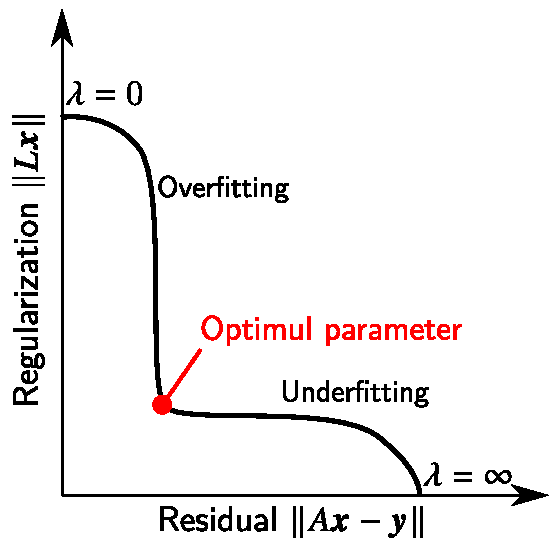
\includegraphics{./regularization/L-curve.pdf}
    \caption{L-curve の概形}
    \label{fig:regularization_l-curve_l-curve}
\end{figure}

正則化の式 \eqref{eq:regularization_intro_general-regularization} を最小化する
$\bm{x}$ を $\bm{x}_\lambda$ として,
横軸を残差 $\|A\bm{x}_\lambda-\bm{y}\|$,
縦軸を正則化項 $R(\bm{x}_\lambda)$ とし,
正則化パラメータ $\lambda$ を変えたときの
プロットを L-curve と呼ぶ.
L-curve は一般に図 \ref{fig:regularization_l-curve_l-curve} のような L の字を
描いている場合が多い.
単純にノルムをプロットするよりも
両対数グラフにプロットする方が
後述する曲線の特徴をはっきりさせられる他,
スケールの違いによる影響を
抑えられるなどのメリットもあるという
\cite{Hansen1998}.

図 \ref{fig:regularization_l-curve_l-curve} のように L-curve が得られた場合,
L の字の曲がり角にあたる赤い点の部分から左上の方では
残差がほとんど減らずに正則化項が増加しており,
右下の方では正則化項がほとんど減らずに残差が増えているため,
両方のバランスが取れている L の字の曲がり角を取るのが良いと考えられる.
そこで,L-curve の曲がり角を数値的に求める手法について考える.

ここでは,文献 \cite{Hansen1998} に従い次の関数の組を考える.
\begin{equation}
    (\xi(\lambda), \eta(\lambda))
    =(\log\|A \bm{x}_\lambda - \bm{y}\|, \log{R(\bm{x})})
\end{equation}
L-curve の曲がり角は曲線 $(\xi(\lambda), \eta(\lambda))$ の
曲率が最も大きい部分と考えられるため,曲率
\begin{equation}
    \kappa(\lambda) =
    \frac{\xi'\eta'' - \xi''\eta'}
    {\left( (\xi')^2 + (\eta')^2 \right)^{3/2}}
    \label{eq:regularization_l-curve_curvature}
\end{equation}
を求め,それを最大化する.
曲率が何らかの手法で求まれば,
1 変数の最適化については
\ref{chap:opt_one-dim-section-search} 章で説明しているため,
ここでは曲率の計算法について考える.

\section{Tikhonov 正則化の場合}

Tikhonov 正則化(\ref{chap:regularization_tikhonov} 章)の場合,
式 \eqref{eq:regularization_l-curve_curvature} にある各種微分を
陽的に表すことができる
\cite{Hansen1992,Mueller2012}.

\begin{align}
    \frac{d}{d\lambda} \|A \bm{x}_\lambda - \bm{y}\|_2^2
     & = \sum_{i=1}^r \frac{2 \lambda \sigma_i^2}{(\sigma_i^2 + \lambda)^3}
    \left(\bm{u}_i^* \bm{y}\right)^2
    \\
    \frac{d}{d\lambda} \|\bm{x}_\lambda\|_2^2
     & = \sum_{i=1}^r \frac{-2 \sigma_i^2}{(\sigma_i^2 + \lambda)^3}
    \left(\bm{u}_i^* \bm{y}\right)^2
    \\
    \frac{d^2}{d\lambda^2} \|A \bm{x}_\lambda - \bm{y}\|_2^2
     & = \sum_{i=1}^r \frac{2 \sigma_i^4 - 4 \lambda \sigma_i^2}
    {(\sigma_i^2 + \lambda)^4}
    \left(\bm{u}_i^* \bm{y}\right)^2
    \\
    \frac{d^2}{d\lambda^2} \|\bm{x}_\lambda\|_2^2
     & = \sum_{i=1}^r \frac{6 \sigma_i^2}{(\sigma_i^2 + \lambda)^4}
    \left(\bm{u}_i^* \bm{y}\right)^2
\end{align}

これらは式
\eqref{eq:regularization_tikhonov_residual-by-svd},
\eqref{eq:regularization_tikhonov_regularization-term-by-svd}
から求めることができる.

% !TEX root = ../main.tex
%

\chapter{Generalized Cross Validation}

正則化パラメータを求めるための手法の 1 つに
Generalized Cross Validation (GCV) がある.
GCV では,次の式の最小化を行う
\cite{Wahba1990}.

\begin{equation}
    V(\lambda)
    = \frac{\frac{1}{m} \|A \bm{x}_\lambda - \bm{y}\|^2}
    {\left|\frac{1}{m} \tr\{I - P_A(\lambda)\}\right|^2}
    \label{eq:regularization_gcv_gcv-evaluation-function}
\end{equation}

ここで,$\bm{x}_\lambda$ は
正則化の式 \eqref{eq:regularization_intro_general-regularization} を最小化する
$\bm{x}$であり,
$P_A(\lambda)$ は influence matrix と呼ばれるもので,
データ $\bm{y}$ から解 $\bm{x}_\lambda$ を求める作用素を $A_\lambda^\#$ としたときに,
\begin{equation}
    P_A(\lambda) \equiv
    \frac{\partial A A_\lambda^\# \bm{y}}{\partial \bm{y}}
    \label{eq:regularization_gcv_influence-matrix}
\end{equation}
のように定義される.

\section{導出}

まず,GCV の基になっている Ordinary Cross Validation (OCV) を
文献 \cite{Wahba1990} に沿って示す.

OCV では次の関数を考える.
\begin{equation}
    V_0(\lambda) \equiv
    \frac{1}{m} \sum_{i=1}^m
    \left|y_i - A_i \bm{x}_\lambda^{(i)}\right|^2
    \label{eq:regularization_gcv_ocv-evaluation-function}
\end{equation}
ただし,$\bm{x}_\lambda^{(i)}$ は $y_i$ 以外のデータから求めた解で,
$A_i$ は解からデータ $y_i$ を推定する作用素である.

ここで次の補題が成り立つ.
\begin{lemma}[文献 {\cite{Wahba1990}} の補題 4.2.1 より, leaving-out-one lemma]
    評価関数
    \begin{equation}
        \frac{1}{m} \left(\left|z - A_k \bm{x}\right|^2
        + \sum_{i \neq k} \left|y_i - A_i \bm{x}\right|^2\right)
        + \lambda R(\bm{x})
    \end{equation}
    を最小化するような $\bm{x}$ を $\bm{h}_\lambda[k,z]$ とし,
    評価関数
    \begin{equation}
        \frac{1}{m}
        \sum_{i \neq k} \left|y_i - A_i \bm{x}\right|^2
        + \lambda R(\bm{x})
    \end{equation}
    を最小化するような $\bm{x}$ を $\bm{x}_\lambda^{(k)}$ としたとき,
    $h_\lambda[k, A_k \bm{x}_\lambda^{(k)}] = \bm{x}_\lambda^{(k)}$
    が成り立つ.
\end{lemma}
\begin{proof}
    $\tilde{y}_k = A_k \bm{x}_\lambda^{(k)}$とし,
    $\bm{x} \neq \bm{x}_\lambda^{(k)}$とする.
    このとき,
    \begin{align}
         & \hphantom{=}
        \frac{1}{m} \left(\left|\tilde{y}_k - A_k \bm{x}_\lambda^{(k)}\right|^2
        + \sum_{i \neq k} \left|y_i - A_i \bm{x}_\lambda^{(k)}\right|^2\right)
        + \lambda R(\bm{x}_\lambda^{(k)})
        \notag                                                                         \\
         & = \frac{1}{m} \sum_{i \neq k} \left|y_i - A_i \bm{x}_\lambda^{(k)}\right|^2
        + \lambda R(\bm{x}_\lambda^{(k)})
        \notag                                                                         \\
         & < \frac{1}{m} \sum_{i \neq k} \left|y_i - A_i \bm{x}\right|^2
        + \lambda R(\bm{x})
        \notag                                                                         \\
         & \le \frac{1}{m} \left(\left|\tilde{y}_k - A_k \bm{x}\right|^2
        +\sum_{i \neq k} \left|y_i - A_i \bm{x}\right|^2\right)
        + \lambda R(\bm{x})
    \end{align}
    のように変形できる.
    よって,
    $h_\lambda[k, A_k \bm{x}_\lambda^{(k)}] = \bm{x}_\lambda^{(k)}$
    である.
\end{proof}

これを用い,次の量を考える.
\begin{equation}
    \tilde{p}_{kk}(\lambda)
    \equiv \frac{A_k \bm{x}_\lambda - A_k \bm{x}_\lambda^{(k)}}
    {y_k - A_k \bm{x}_\lambda^{(k)}}
\end{equation}
まず,定義から,
\begin{equation}
    y_k - A_k \bm{x}_\lambda^{(k)} =
    \frac{y_k - A_k \bm{x}_\lambda}{1 - \tilde{p}_{kk}(\lambda)}
\end{equation}
が成り立つ.
また,補題から
\begin{equation}
    \tilde{p}_{kk}(\lambda)
    = \frac{A_k h[k,y_k] - A_k h[k,\tilde{y}_k]}{y_k - \tilde{y}_k}
\end{equation}
が成り立つ.
さらに,これは 1 次近似により
\begin{equation}
    \tilde{p}_{kk}(\lambda)
    \approx \frac{\partial A_k h[k,y_k]}{\partial y_k}
    =\frac{\partial A_k \bm{x}_\lambda}{\partial y_k}
    =\frac{\partial A_k A_\lambda^\# \bm{y}}{\partial y_k}
    =p_{kk}(\lambda)
\end{equation}
と書ける.
ただし,$p_{kk}(\lambda)$ は
influence matrix $P_A(\lambda)$ の $(k,k)$ 成分である.

このことを利用して OCV の評価関数
\eqref{eq:regularization_gcv_ocv-evaluation-function}
を変形すると,
\begin{equation}
    V_0(\lambda)=
    \frac{1}{m} \sum_{i=1}^m
    \left|y_i - A_i \bm{x}_\lambda^{(i)}\right|^2
    \approx
    \frac{1}{m} \sum_{i=1}^m
    \frac{\left|y_i - A_i \bm{x}_\lambda\right|^2}
    {\left|1 - p_{kk}(\lambda)\right|^2}
\end{equation}
のように書ける.

$p_{kk}(\lambda)$
の代わりに,influence matrix の対角成分の平均値
$\tr P_A(\lambda)/n$
を用い,
$\bm{y}$
の回転に影響されない評価関数を作ると,
GCVの評価関数 \eqref{eq:regularization_gcv_gcv-evaluation-function} が得られる.

\section{Tikhonov 正則化の場合における計算方法}

Tikhonov 正則化(\ref{chap:regularization_tikhonov} 章)の場合,
残差項は式 \eqref{eq:regularization_tikhonov_residual-by-svd} で計算できる.
そこで,influence matrix の計算について考える.

\ref{chap:regularization_tikhonov} 章と同様に
行列 $A$ の特異値分解
\begin{equation}
    A = U
    \begin{pmatrix}
        \Sigma & O \\
        O      & O
    \end{pmatrix}
    V^*
\end{equation}
を行い,その場合の解(式 \eqref{eq:regularization_tikhonov_solution-by-svd-matrices})
\begin{equation}
    x_{\lambda} = V
    \begin{pmatrix}
        (\Sigma^2 + \lambda I)^{-1} \Sigma & O \\
        O                                  & O
    \end{pmatrix}
    U^* \bm{y}
\end{equation}
を利用すると,
\begin{align}
    A A_\lambda^\# \bm{y}
     & = U
    \begin{pmatrix}
        \Sigma & O \\
        O      & O
    \end{pmatrix}
    V^* V
    \begin{pmatrix}
        (\Sigma^2 + \lambda I)^{-1} \Sigma & O \\
        O                                  & O
    \end{pmatrix}
    U^* \bm{y}
    \notag \\
     & = U
    \begin{pmatrix}
        \Sigma (\Sigma^2 + \lambda I)^{-1} \Sigma & O \\
        O                                         & O
    \end{pmatrix}
    U^* \bm{y}
\end{align}
となる.
よって,influence matrix は
\begin{align}
    P_A(\lambda)
     & = \frac{\partial A A_\lambda^\# \bm{y}}{\partial \bm{y}}
    \notag                                                      \\
     & = U
    \begin{pmatrix}
        \Sigma (\Sigma^2 + \lambda I)^{-1} \Sigma & O \\
        O                                         & O
    \end{pmatrix}
    U^*
\end{align}
であり,そのトレースは
\begin{align}
    \tr{P_A(\lambda)}
     & = \tr\left(U
    \begin{pmatrix}
            \Sigma (\Sigma^2 + \lambda I)^{-1} \Sigma & O \\
            O                                         & O
        \end{pmatrix}
    U^*\right)
    \notag                                                      \\
     & = \tr\left(
    \begin{pmatrix}
            \Sigma (\Sigma^2 + \lambda I)^{-1} \Sigma & O \\
            O                                         & O
        \end{pmatrix}
    U^* U\right)
    \notag                                                      \\
     & = \tr
    \begin{pmatrix}
        \Sigma (\Sigma^2 + \lambda I)^{-1} \Sigma & O \\
        O                                         & O
    \end{pmatrix}
    \notag                                                      \\
     & = \sum_{i = 1}^r \frac{\sigma_i^2}{\sigma_i^2 + \lambda}
\end{align}
と計算できる
\cite{Hansen1998}
\footnote{$\sigma_i^2 / (\sigma_i^2 + \lambda)$ は filter factor と呼ばれる.}.

\section{一般の場合における計算方法}

解きたい方程式や正則化項が非線形な場合,
反復的な最適化アルゴリズムで正則化した推定解を求めることになるが,
そのような場合の GCV をどのように計算すれば良いのかについて,
文献 \cite{Deshpande1991} の結果を簡単に紹介する.
なお,本節では,データ $\bm{y}$ が実数であることを前提とする.

まず,非線形な問題においてどのような問題が起きるかをまとめる.
式 \eqref{eq:regularization_gcv_gcv-evaluation-function} で示した GCV の評価関数において,
分子は推定解 $\bm{x}_\lambda$ における残差であり,計算できる場合が多い.
それに対して分母は
推定解に $A$ を作用した結果 $A A_\lambda^\#\bm{y}$ を
$\bm{y}$ について偏微分したヤコビアン $P_A(\lambda)$ を含んでおり,
非線形な問題においてはこれを解析的に計算することができない.
数値的にこれを求めることも可能だが,
その場合は全ての $i=1, 2, \ldots, n$ について
$i$ 要素目だけ1の単位行列 $\bm{e}_i$ ($i$ の要素だけ 1 の単位ベクトル)の方向へデータをずらした
$\bm{y} + \Delta y_i \bm{e}_i$ について推定解を得て
$A$ を作用させることにより,
数値微分する必要がある.
これは推定解を求めるのに時間のかかる最適化において現実的ではない.
この問題を解決するために,
文献 \cite{Deshpande1991} では次のような2段階の近似を行っている.

まず,分母を次の式で近似する.
\begin{align}
    \frac{1}{m} \tr(I - P_A(\lambda))
     & \approx \frac{\bm{w}^T (I - P_A(\lambda)) \bm{w}}{\bm{w}^T \bm{w}}
    \label{eq:regularization_gcv_influence-approximation-by-Deshpande}
\end{align}
これは文献 \cite{Girard1989} において提案された
Monte-Carlo Cross-Validation と呼ばれる手法のもので,
$\bm{w}$ は各要素を独立に平均 0,分散 1 の正規分布 $\mathcal{N}(0,1)$ から
サンプリングしたベクトルである.
なお,この手法は線形
(つまり $P_A(\lambda) = A A_\lambda^\#$ と行列で書ける)
だが大規模な問題を解くために考えられたもので,
そのような問題では,たとえ $P_A(\lambda)$ が陽的に書けても,
トレース $\tr(I - P_A(\lambda))$ を計算するのは
かなりコストを要するという問題があり,
このような手法が考案された.
この近似式については次のような定理が証明されている.

\begin{theorem}[文献{\cite{Girard1989}} 定理 2.2]
    行列 $B \in \setR^{m \times m}$ と
    各要素が独立に正規分布 $\mathcal{N}(0,1)$ に従う
    ベクトル $\bm{w} \in \setR^m$ を用いて
    \begin{equation}
        T_B^*(\bm{w}) \equiv \frac{\bm{w}^T B \bm{w}}{\bm{w}^T \bm{w}}
    \end{equation}
    を定義する.
    このとき,$T_B^*$ の平均と分散はそれぞれ
    \begin{align}
        \mathrm{E}[T_B^*(\bm{w})]   & =\mu_1 \equiv \frac{1}{m} \tr(B) = \frac{1}{m} \sum_{i=1}^m B_{ii}
        \\
        \mathrm{Var}[T_B^*(\bm{w})] & =\frac{2}{m (m + 2)} \sum_{i=1}^m (B_{ii} - \mu_1)^2
    \end{align}
    となる.
\end{theorem}

ここで出てくる分散による誤差が気になる場合は,
複数の $\bm{w}$ で
式 \eqref{eq:regularization_gcv_influence-approximation-by-Deshpande} の近似を行った
結果の平均で $\tr(I-P_A(\lambda))/n$ の推定を行うことで
精度を上げることもできる.
しかし,文献 \cite{Girard1989} の数値実験では
$m=50$ でも真値と似たような挙動をとる推定値が得られており,
$m=500$ では真値との差をグラフから読み取るのが困難な程度に良い結果が得られている.

文献 \cite{Deshpande1991} では
\begin{align}
    P_A(\lambda) \bm{w}
     & = \frac{\partial A A_\lambda^\# \bm{y}}{\partial \bm{y}} \bm{w}
    \notag                                                                   \\
     & \approx \frac{AA_\lambda^\#(\bm{y}+h\bm{w}) - AA_\lambda^\#\bm{y}}{h}
\end{align}
と近似することで,次の式を得ている.

\begin{align}
    \frac{1}{m} \tr(I - P_A(\lambda))
     & \approx \frac{\bm{w}^T (I - P_A(\lambda)) \bm{w}}{\bm{w}^T \bm{w}}
    \notag                                                                \\
     & = \frac{\bm{w}^T}{\bm{w}^T \bm{w}}(\bm{w} - P_A(\lambda) \bm{w})
    \notag                                                                \\
     & \approx \frac{\bm{w}^T}{\bm{w}^T \bm{w}}
    \left(\bm{w} - \frac{A A_\lambda^\#(\bm{y} + h \bm{w}) - A A_\lambda^\# \bm{y}}{h}\right)
\end{align}

数値微分のずらす幅を決める $h$ は
$A A_\lambda^\#$ の演算の精度を見ながら調整することになるが,
これにより推定解の計算を最低 2 回行えば GCV の評価関数を計算できる.

